% 指数関数 y = 2^x と y = (1/2)^x のグラフ（CC BY-SA 4.0）
\begin{tikzpicture}[scale=0.62]
  \draw[step=1,black!12] (-3.4,-0.4) grid (3.4,6.4);
  \draw[->] (-3.6,0) -- (3.7,0) node[right] {$x$};
  \draw[->] (0,-0.6) -- (0,6.7) node[above] {$y$};
  \foreach \t in {-3,-2,-1,1,2,3} \node[below,font=\scriptsize] at (\t,0) {$\t$};
  \node[below left,font=\scriptsize] at (0,0) {O};
  \foreach \t in {2,4,6} \node[left,font=\scriptsize] at (0,\t) {$\t$};
  \draw[very thick,blue,domain=-3.4:2.6,samples=60] plot (\x,{2^\x});
  \draw[very thick,red,domain=-2.6:3.4,samples=60] plot (\x,{2^(-\x)});
  \node[blue,right] at (2.55,5.9) {$y = 2^x$};
  \node[red,left] at (-2.55,5.9) {$y = \left(\tfrac12\right)^x$};
  \fill (0,1) circle (3pt);
  \draw[->,thin] (1.05,1.55) -- (0.12,1.05);
  \node[right,font=\small,fill=white,inner sep=1pt] at (1.05,1.55) {$(0,\,1)$};
\end{tikzpicture}
